% ============================================================
%  يُترجَم بـ XeLaTeX  (في Overleaf: Menu → Compiler → XeLaTeX)
%  الخط: Amiri (متوفر في Overleaf، أو حمّله من github.com/aliftype/amiri)
% ============================================================
\documentclass[12pt,a4paper]{article}
\usepackage[a4paper,margin=1.2cm,top=2.3cm,bottom=2.9cm,headheight=15pt,footskip=1.5cm]{geometry}
\usepackage{amsmath,amssymb}
\usepackage{icomma}
\usepackage[english,bidi=default,layout=lists]{babel}
\babelprovide[import,main]{arabic}
\babelfont{rm}[Scale=1.08]{Amiri}
\babelfont{sf}[Scale=1.08]{Amiri}
\usepackage[most]{tcolorbox}
\usepackage{tikz}
\usetikzlibrary{arrows.meta,calc,shadings}
\usepackage{array}
\usepackage{colortbl}
\usepackage{fancyhdr}
\usepackage{titlesec}
\usepackage{enumitem}
\usepackage{collcell}
\usepackage{needspace}
\usepackage{etoolbox}
\newcolumntype{C}{>{\collectcell\ar}c<{\endcollectcell}}
\pretocmd{\section}{\Needspace{15\baselineskip}}{}{}
\pretocmd{\subsection}{\Needspace{11\baselineskip}}{}{}

\definecolor{cDef}{HTML}{1F4E9C}
\definecolor{cThm}{HTML}{B3261E}
\definecolor{cRem}{HTML}{2E7D32}
\definecolor{cEx}{HTML}{C76B00}
\definecolor{cMeth}{HTML}{6A1B9A}
\definecolor{cSol}{HTML}{00695C}
\definecolor{cSec}{HTML}{1F3A68}

\titleformat{\section}{\Large\bfseries\color{cSec}}{\thesection.}{0.6em}{}[{\color{cSec!60}\titlerule[1pt]}]
\titleformat{\subsection}{\large\bfseries\color{cThm!85!black}}{\thesubsection.}{0.5em}{}
\titlespacing*{\section}{0pt}{14pt}{8pt}
\titlespacing*{\subsection}{0pt}{10pt}{5pt}
\setlength{\parindent}{0pt}
\setlength{\parskip}{4pt}
\setlist{itemsep=2pt,topsep=3pt}

\newtcolorbox{arbox}[3][]{enhanced,
  colback=#2!5,colframe=#2!80!black,arc=2mm,boxrule=0.8pt,
  left=6pt,right=6pt,top=8pt,bottom=5pt,
  fonttitle=\bfseries,coltitle=white,
  title={\foreignlanguage{arabic}{#3}},
  attach boxed title to top right={xshift=-5mm,yshift=-3mm},
  boxed title style={colback=#2!80!black,arc=1.5mm,boxrule=0pt},
  before upper={\selectlanguage{arabic}},
  before skip=8pt,after skip=8pt,breakable,#1}
\newenvironment{BOX}[2]{\begin{otherlanguage}{english}\begin{arbox}{#1}{#2}}{\end{arbox}\end{otherlanguage}}
\newenvironment{tarif}[1][تعريف]{\begin{BOX}{cDef}{#1}}{\end{BOX}}
\newenvironment{khassia}[1][خاصية]{\begin{BOX}{cThm}{#1}}{\end{BOX}}
\newenvironment{molahada}[1][ملاحظة]{\begin{BOX}{cRem}{#1}}{\end{BOX}}
\newenvironment{mithal}[1][مثال]{\begin{BOX}{cEx}{#1}}{\end{BOX}}
\newenvironment{tariqa}[1][طريقة]{\begin{BOX}{cMeth}{#1}}{\end{BOX}}

\newcounter{exo}
\newenvironment{tamrin}[1]{\stepcounter{exo}\begin{BOX}{cSec}{التمرين \theexo: #1}}{\end{BOX}}
\newenvironment{hal}{\Needspace{12\baselineskip}\begin{otherlanguage}{english}\begin{arbox}[breakable]{cSol}{حل التمرين \theexo}}{\end{arbox}\end{otherlanguage}}

\newenvironment{LTR}{\begin{otherlanguage}{english}}{\end{otherlanguage}}
\newcommand{\ar}[1]{\foreignlanguage{arabic}{#1}}

\renewcommand{\dots}{\mathinner{\ldotp\ldotp\ldotp}}
\renewcommand{\ldots}{\mathinner{\ldotp\ldotp\ldotp}}
\renewcommand{\cdots}{\mathinner{\cdotp\cdotp\cdotp}}
\newcommand{\N}{\mathbb{N}}
\newcommand{\Z}{\mathbb{Z}}
\newcommand{\D}{\mathbb{D}}
\newcommand{\Q}{\mathbb{Q}}
\newcommand{\R}{\mathbb{R}}
\newcommand{\pgcd}{\operatorname{PGCD}}
\newcommand{\ppcm}{\operatorname{PPCM}}

% \NLseg{a}{b}{[}{]} ; \NLright{a}{[} ; \NLleft{b}{]}  (interval on a number line)
\newcommand{\NLseg}[4]{\begin{LTR}\begin{tikzpicture}[baseline=-0.6ex]
 \draw[-{Stealth[length=2mm]},gray!70](0,0)--(3.4,0);
 \draw[line width=2pt,cThm!80!black](0.7,0)--(2.7,0);
 \node[cThm!80!black,font=\LARGE] at (0.7,0){$#3$};
 \node[cThm!80!black,font=\LARGE] at (2.7,0){$#4$};
 \node[below=3pt,font=\footnotesize] at (0.7,0){$#1$};
 \node[below=3pt,font=\footnotesize] at (2.7,0){$#2$};
\end{tikzpicture}\end{LTR}}
\newcommand{\NLright}[2]{\begin{LTR}\begin{tikzpicture}[baseline=-0.6ex]
 \draw[-{Stealth[length=2mm]},gray!70](0,0)--(3.4,0);
 \draw[line width=2pt,cThm!80!black](1.3,0)--(3.3,0);
 \node[cThm!80!black,font=\LARGE] at (1.3,0){$#2$};
 \node[below=3pt,font=\footnotesize] at (1.3,0){$#1$};
\end{tikzpicture}\end{LTR}}
\newcommand{\NLleft}[2]{\begin{LTR}\begin{tikzpicture}[baseline=-0.6ex]
 \draw[-{Stealth[length=2mm]},gray!70](0,0)--(3.4,0);
 \draw[line width=2pt,cThm!80!black](0.05,0)--(2.1,0);
 \node[cThm!80!black,font=\LARGE] at (2.1,0){$#2$};
 \node[below=3pt,font=\footnotesize] at (2.1,0){$#1$};
\end{tikzpicture}\end{LTR}}

% ---------- social-media icons (pure TikZ) ----------
\definecolor{cFB}{HTML}{1877F2}
\definecolor{cTG}{HTML}{229ED9}
\definecolor{cIG1}{HTML}{FEDA75}
\definecolor{cIG2}{HTML}{D62976}
\definecolor{cIG3}{HTML}{4F5BD5}
\newcommand{\fbicon}{\begin{LTR}\begin{tikzpicture}[baseline=-0.75ex,x=1em,y=1em]
 \fill[cFB] (0,0) circle (0.55);
 \node[white,inner sep=0,font=\usefont{TU}{lmss}{bx}{n}\small] at (0.04,-0.02) {f};
\end{tikzpicture}\end{LTR}}
\newcommand{\igicon}{\begin{LTR}
\begin{tikzpicture}[baseline=-0.75ex,x=1em,y=1em]
 \shade[lower left=cIG1,lower right=cIG2,upper left=cIG2,upper right=cIG3,rounded corners=0.28em] (-0.55,-0.55) rectangle (0.55,0.55);
 \draw[white,line width=0.09em,rounded corners=0.18em] (-0.36,-0.36) rectangle (0.36,0.36);
 \draw[white,line width=0.09em] (0,0) circle (0.17);
 \fill[white] (0.22,0.22) circle (0.05);
\end{tikzpicture}\end{LTR}}
\newcommand{\tgicon}{\begin{LTR}
\begin{tikzpicture}[baseline=-0.75ex,x=1em,y=1em]
 \fill[cTG] (0,0) circle (0.55);
 \fill[white] (-0.33,0.0) -- (0.32,0.27) -- (0.2,-0.3) -- (0.0,-0.15) -- (-0.08,-0.28) -- (-0.08,-0.08) -- cycle;
 \fill[cTG!70!black] (-0.08,-0.08) -- (0.25,0.2) -- (0.0,-0.15) -- (-0.08,-0.28) -- cycle;
\end{tikzpicture}\end{LTR}}
% page number: black box, white two-digit number, at the right of the social row
\newcommand{\PageBox}{\begin{LTR}\tikz[baseline=(p.base)]\node[fill=black,text=white,inner sep=2.5pt,minimum width=1.6em,minimum height=1.3em,font=\usefont{TU}{lmss}{bx}{n}\small](p){\ifnum\value{page}<10 0\fi\arabic{page}};\end{LTR}}
% visual left-to-right order: Telegram | Instagram | Facebook | page box
\newcommand{\SocialRow}{\begin{otherlanguage}{english}%
 \ar{\textbf{الأستاذ سوايسية هشام للرياضيات}}\ \tgicon\hfill
 \textbf{prof\_hicham\_math}\ \igicon\hfill
 \ar{\textbf{الأستاذ سوايسية هشام للرياضيات}}\ \fbicon\hspace{2.2em}\PageBox\end{otherlanguage}}

\pagestyle{fancy}
\fancyhf{}
\renewcommand{\headrulewidth}{0.6pt}
\renewcommand{\footrulewidth}{0.4pt}
% \SetHeader{right head: document title}{left head: level -- stream}
\newcommand{\SetHeader}[2]{%
 \fancyhead[C]{\parbox{\textwidth}{\ar{#1\hfill #2}}}%
 \fancyfoot[C]{\parbox{\textwidth}{\small\SocialRow}}}
\usepackage{tkz-tab}
\usepackage{multicol}
% variation / sign table (LTR)
\newenvironment{TAB}{\par\begin{center}\begin{LTR}\begin{tikzpicture}[scale=0.95,every node/.style={font=\small}]}{\end{tikzpicture}\end{LTR}\end{center}}
% grid + axes, clipped: \begin{GR}{xmin}{xmax}{ymin}{ymax}{unit cm}
\newenvironment{GR}[5]{\par\begin{center}\begin{LTR}\begin{tikzpicture}[x=#5cm,y=#5cm,font=\footnotesize]
 \draw[gray!25,very thin] (#1,#3) grid (#2,#4);
 \draw[-{Stealth[length=2mm]}] (#1,0)--(#2+0.3,0) node[below left]{$x$};
 \draw[-{Stealth[length=2mm]}] (0,#3)--(0,#4+0.3) node[below left]{$y$};
 \node[below left] at (0,0){$O$};
 \begin{scope}\clip (#1,#3) rectangle (#2,#4);}
{\end{scope}\end{tikzpicture}\end{LTR}\end{center}}
\newcommand{\Ticks}[2]{\foreach \t in {#1} \node[below,font=\scriptsize] at (\t,0){$\t$}; \foreach \t in {#2} \node[left,font=\scriptsize] at (0,\t){$\t$};}
\newcommand{\bx}[1]{\ensuremath{\colorbox{cDef!12}{$\displaystyle #1$}}}
\newcommand{\TwoCol}[4]{\par\begin{LTR}\noindent\begin{minipage}[t]{#1\textwidth}\selectlanguage{arabic}#2\end{minipage}\hfill\begin{minipage}[t]{#3\textwidth}\selectlanguage{arabic}#4\end{minipage}\end{LTR}\par}
\newcommand{\RL}[4]{\TwoCol{#3}{#4}{#1}{#2}}  % \RL{w1}{right content}{w2}{left content}
\newcommand{\ok}{$\textcolor{cRem}{\checkmark}$}
\newcommand{\limn}{\displaystyle\lim_{n\to+\infty}}
% sub-questions, each on its own line
\newenvironment{sq}{\begin{itemize}[leftmargin=2.4em,itemsep=3pt]}{\end{itemize}}
\newcommand{\qa}{\item[(أ)]}\newcommand{\qb}{\item[(ب)]}\newcommand{\qc}{\item[(جـ)]}\newcommand{\qd}{\item[(د)]}\newcommand{\qe}{\item[(هـ)]}
\newcommand{\pa}{\par\smallskip\textbf{(أ)} }\newcommand{\pb}{\par\smallskip\textbf{(ب)} }\newcommand{\pc}{\par\smallskip\textbf{(جـ)} }\newcommand{\pd}{\par\smallskip\textbf{(د)} }\newcommand{\pe}{\par\smallskip\textbf{(هـ)} }
\newcommand{\QQ}[1]{\par\smallskip\textbf{#1.} }
\newenvironment{tmr}{\stepcounter{exo}\begin{BOX}{cSec}{تمرين محلول \theexo}}{\end{BOX}}
\newcommand{\ABC}[3]{\\[2pt]\begin{tabular}{p{0.28\textwidth}p{0.28\textwidth}p{0.28\textwidth}}(جـ) \ #3 & (ب) \ #2 & (أ) \ #1\end{tabular}}
\pretocmd{\section}{\Needspace{24\baselineskip}}{}{}
\newtcbox{\bxtbox}{on line,colback=cDef!12,colframe=cDef!12,boxrule=0pt,arc=1pt,boxsep=0pt,left=2pt,right=2pt,top=1pt,bottom=1pt}
\newcommand{\bxt}[1]{\foreignlanguage{english}{\bxtbox{\ar{#1}}}}
\usepackage{longtable}
\setlength{\LTpre}{4pt}\setlength{\LTpost}{0pt}
\newcommand{\Phase}[1]{\textbf{#1}}
\newcommand{\Fld}[2]{\textbf{#1:}\ #2}
% رأس المذكرة على نمط النموذج: إطار بعنوان «مذكرة رقم»، معلومات الحصة، ثم إطار الكفاءات
\newcommand{\ModhHead}[9]{%
\begin{LTR}
\begin{tcolorbox}[enhanced,colback=white,colframe=cThm!85!black,arc=4mm,boxrule=1pt,top=14pt,bottom=6pt,left=8pt,right=8pt,
 overlay={\node[fill=cThm!85!black,text=white,rounded corners=3mm,inner xsep=14pt,inner ysep=4pt,font=\large\bfseries] at ([yshift=0pt]frame.north){\ar{مذكرة رقم #1}};},
 before upper={\selectlanguage{arabic}}]
\begin{tabular}{@{}p{0.4\linewidth}p{0.55\linewidth}@{}}
\Fld{المستوى}{#2} & \Fld{الثانوية}{\dotfill}\\[3pt]
\Fld{المادة}{رياضيات} & \Fld{ميدان التعلم}{#3}\\[3pt]
\Fld{المدة}{#5} & \Fld{الوحدة التعلمية}{#4}\\[3pt]
\Fld{الأستاذ}{\dotfill} & \Fld{المحتوى المعرفي}{#6}\\
\end{tabular}
\end{tcolorbox}
\begin{tcolorbox}[enhanced,colback=white,colframe=cThm!85!black,arc=3mm,boxrule=0.8pt,sidebyside,sidebyside align=top,lefthand ratio=0.5,
 segmentation style={dashed,cThm!60},before upper={\selectlanguage{arabic}},before lower={\selectlanguage{arabic}}]
\textbf{الكفاءات المستهدفة:}\par #8
\tcblower
\textbf{الكفاءات القبلية:}\par #7
\end{tcolorbox}
\end{LTR}
\par\smallskip\textbf{الوسائل:} #9\par\smallskip}
\newenvironment{Sayr}{%
\begin{LTR}\renewcommand{\arraystretch}{1.25}\setlength{\tabcolsep}{4pt}\relpenalty=10000\binoppenalty=10000\tolerance=9000\emergencystretch=0.3\linewidth
\begin{longtable}{|p{0.09\textwidth}|>{\centering\arraybackslash}p{0.05\textwidth}|p{0.71\textwidth}|>{\centering\arraybackslash}p{0.09\textwidth}|}
\hline\rowcolor{cThm!12}\ar{\footnotesize\textbf{توجيهات وتعاليق}} & \ar{\footnotesize\textbf{المدة}} & \ar{\textbf{سير الحصة}} & \ar{\footnotesize\textbf{مراحل الحصة}}\\\hline\endhead
\hline\endfoot}{\end{longtable}\end{LTR}}
% سطر في الجدول: \Row{مرحلة}{سير}{مدة}{توجيهات}
\newcommand{\RaggedEnd}{\leftskip=0pt plus 1fil\relax}
\newcommand{\Row}[4]{\ar{\small #4} & \ar{#3} & \ar{\RaggedEnd #2} & \cellcolor{cThm!8}\ar{\Phase{#1}}\\\hline}

\newcommand{\Lab}[2]{\foreignlanguage{english}{\tcbox[on line,colback=#1,colframe=#1,boxrule=0pt,arc=2pt,boxsep=1pt,left=5pt,right=5pt,top=1pt,bottom=1pt]{\ar{\textcolor{white}{\textbf{#2}}}}}}
\newcommand{\Num}[1]{\foreignlanguage{english}{\tikz[baseline=(c.base)]\node[fill=cDef,text=white,inner sep=2pt,font=\footnotesize\bfseries](c){#1};}}
\newcommand{\ck}{\ensuremath{{\color{cRem}\checkmark}}}
\newenvironment{Kad}[1]{\par\smallskip\Lab{#1}}{\par}
\newcommand{\RR}[1]{\ifmmode{\color{cThm}#1}\else$\mbox{\color{cThm}#1}$\fi}
\newcommand{\T}[1]{$\mbox{\color{cDef}\bfseries #1}$}
\SetHeader{\small\bfseries\color{cSec}مذكرات محور: الدالة اللوغاريتمية النيبيرية}{\small\color{cSec}السنة الثالثة ثانوي -- علوم تجريبية}
\begin{document}
\begin{LTR}
\begin{tcolorbox}[enhanced,colback=cThm!85!black,colframe=cThm!85!black,arc=3mm,halign=center,boxrule=0pt,top=12pt,bottom=12pt,before upper={\selectlanguage{arabic}}]
{\color{white}\fontsize{24}{30}\selectfont\bfseries مذكرات محور: الدالة اللوغاريتمية النيبيرية}\\[8pt]
{\color{white}\large السنة الثالثة ثانوي -- علوم تجريبية}\\[4pt]
{\color{white}\large 4 مذكرات (8 ساعات) -- السنة الدراسية 2026-2027}
\end{tcolorbox}
\end{LTR}
\begin{BOX}{cThm}{يتضمن هذا العمل}
\begin{enumerate}[label=\textbf{مذكرة \arabic{enumi}:},leftmargin=6em,start=14]
\item الدالة اللوغاريتمية: تعريف ، اتجاه التغير ، معادلات ومتراجحات.
\item الخواص الجبرية للدالة اللوغاريتمية.
\item اشتقاقية الدالة $\ln$ ودراسة الدالة $\ln\circ u$.
\item اللوغاريتم العشري وتطبيقاته.
\end{enumerate}
الحلول مفصّلة: المعطيات بالأسود ، \T{العناوين} و\RR{النتائج} بلون مختلف ، وكل سؤال في سطر.
\end{BOX}
\newpage
\ModhHead{14}{3 ع ت}{تحليل}{الدالة اللوغاريتمية النيبيرية}{02 سا}{الدالة اللوغاريتمية النيبيرية: تعريف ، اتجاه التغير ، معادلات ومتراجحات}%
{\begin{itemize}\item الدالة الأسية: خواصها واتجاه تغيرها ، مبرهنة القيم المتوسطة.\end{itemize}}%
{\begin{itemize}\item تعريف الدالة $\ln$ ومعرفة خواصها المميزة.\item حل معادلات ومتراجحات تتضمن $\ln$.\end{itemize}}%
{المنهاج ، الكتاب المدرسي ، الآلة الحاسبة العلمية ، برمجية Geogebra.}
\begin{Sayr}
\Row{مرحلة الانطلاق}{%
\textbf{التهيئة النفسية:} التذكير بمبرهنة القيم المتوسطة ، وبأن $e^x>0$ وأن الدالة الأسية متزايدة تمامًا.}{10 د}{تذكير.}
\Row{التشخيص والاكتشاف}{%
\Lab{cEx}{نشاط رقم 05}\ (نشاط 2 صفحة 22) نقبل أنه من أجل كل عدد حقيقي $a>0$ توجد قيمة وحيدة $b$ حيث $e^b=a$.\par\textbf{(1)} عيّن العدد $b$ في الحالات: $a=1$ ، $a=e$ ، $a=\dfrac1e$ ، $a=e^2$.\par\textbf{(2)} بالآلة الحاسبة ، عيّن قيمة تقريبية إلى $10^{-3}$ للعدد $b$ حيث $e^b=2$.\par\textbf{(3)} إذا كان $e^{b}=2$ فما العدد $b^{\prime}$ حيث $e^{b^{\prime}}=\dfrac12$ ؟\par\textbf{(4)} بيّن أن النقطة $M(a;b)$ هي نظيرة النقطة $N(b;a)$ من منحنى الدالة الأسية بالنسبة إلى المستقيم $y=x$.}{35 د}{مناقشة النشاط من طرف التلاميذ.}
\Row{}{%
\Lab{cDef}{مناقشة النشاط}\par\textbf{(1)} $e^0=1$ إذن $b=\RR{0}$ ؛ $e^1=e$ إذن $b=\RR{1}$ ؛ $e^{-1}=\dfrac1e$ إذن $b=\RR{-1}$ ؛ $e^2=e^2$ إذن $b=\RR{2}$.\par\textbf{(2)} $e^{0{,}693}\approx2{,}000$ ، إذن $b\approx\RR{0{,}693}$ (لاحظ $0<b<1$ لأن $e^0=1<2<e$).\par\textbf{(3)} $e^{-b}=\dfrac1{e^b}=\dfrac12$ ، إذن $b^{\prime}=\RR{-b}$.\par\textbf{(4)} $e^b=a$ يعني $N(b;a)$ على منحنى الأسية ، و $M(a;b)$ نظيرتها بالنسبة إلى $y=x$: المنحنيان \RR{متناظران}.}{}{}
\Row{بناء المعارف}{%
\Lab{cDef}{تعريف}\ من أجل كل عدد حقيقي $a$ من $]0;+\infty[$ يوجد عدد حقيقي وحيد $b$ حيث $e^b=a$ ، يسمى \textbf{اللوغاريتم النيبيري} للعدد $a$ ونرمز له $\RR{\ln a}$.\par \textbf{الدالة اللوغاريتمية النيبيرية} $\ln$ هي الدالة التي ترفق بكل $x$ من $]0;+\infty[$ العدد $\ln x$.}{50 د}{ربط النشاط بالمفهوم.}
\Row{}{%
\Lab{cRem}{نتائج}\par\textbf{(1)} من أجل $x>0$ و $y\in\mathbb R$: $\RR{\ln x=y}$ يعني $\RR{x=e^y}$.\par\textbf{(2)} من أجل $x>0$: $\RR{e^{\ln x}=x}$ ؛ ومن أجل كل $x$ من $\mathbb R$: $\RR{\ln\left(e^x\right)=x}$.\par\textbf{(3)} $\RR{\ln1=0}$ و $\RR{\ln e=1}$.}{}{}
\Row{}{%
\Lab{cThm}{خاصية}\ الدالة $\ln$ \RR{متزايدة} \RR{تمامًا} \RR{على} \RR{$]0;+\infty[$}.}{}{}
\Row{}{%
\Lab{cMeth}{البرهان}\ ليكن $0<a<b$: $e^{\ln a}<e^{\ln b}$ ، وبما أن الدالة الأسية متزايدة تمامًا فإن $\ln a<\ln b$.}{}{}
\Row{}{%
\Lab{cRem}{نتائج}\ من أجل كل $x>0$ و $y>0$:\par\textbf{(1)} $\RR{\ln x=\ln y}$ يعني $\RR{x=y}$ ؛ $\RR{\ln x<\ln y}$ يعني $\RR{x<y}$.\par\textbf{(2)} $\ln x>0$ يعني $x>1$ ؛ $\ln x<0$ يعني $0<x<1$.}{}{}
\Row{}{%
\Lab{cEx}{جدول التغيرات والتمثيل البياني}\par\smallskip\begin{LTR}\centering 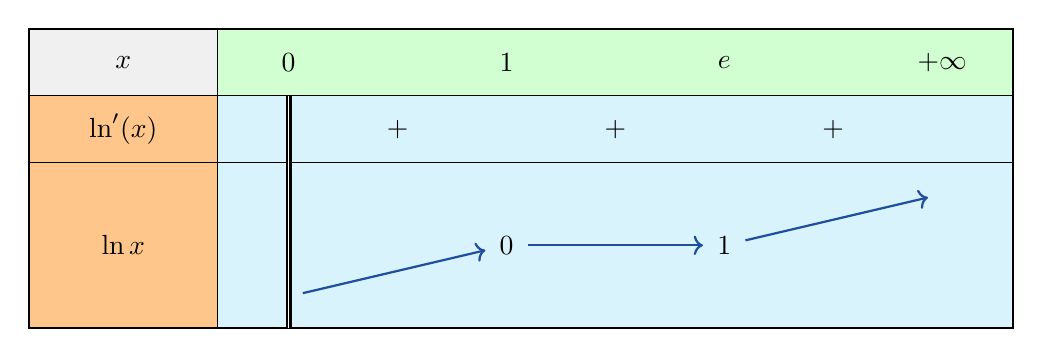
\begin{tikzpicture}[font=\normalsize]
\fill[gray!12] (0,0) rectangle (2.4,-0.85); \fill[green!18] (2.4,0) rectangle (12.5,-0.85);
\fill[orange!45] (0,-0.85) rectangle (2.4,-3.8); \fill[cyan!15] (2.4,-0.85) rectangle (12.5,-3.8);
\draw[thick] (0,0) rectangle (12.5,-3.8); \draw (0,-0.85)--(12.5,-0.85) (0,-1.7)--(12.5,-1.7) (2.4,0)--(2.4,-3.8);
\node at (1.2,-0.425){$x$}; \node at (1.2,-1.275){$\ln^{\prime}(x)$}; \node at (1.2,-2.75){$\ln x$};
\node at (3.3,-0.425){$0$};
\node at (6.06667,-0.425){$1$};
\node at (8.83333,-0.425){$e$};
\node at (11.6,-0.425){$+\infty$};
\draw[double,thick] (3.3,-0.85)--(3.3,-3.8);
\node at (4.68333,-1.275){$+$};
\node at (7.45,-1.275){$+$};
\node at (10.2167,-1.275){$+$};
\node[inner sep=2pt] (v0) at (3.3,-3.4){$$};
\node[inner sep=2pt] (v1) at (6.06667,-2.75){$0$};
\node[inner sep=2pt] (v2) at (8.83333,-2.75){$1$};
\node[inner sep=2pt] (v3) at (11.6,-2.1){$$};
\draw[->,cDef,thick,shorten <=3pt,shorten >=3pt] (v0)--(v1);
\draw[->,cDef,thick,shorten <=3pt,shorten >=3pt] (v1)--(v2);
\draw[->,cDef,thick,shorten <=3pt,shorten >=3pt] (v2)--(v3);
\end{tikzpicture}\end{LTR}\par \par\smallskip\begin{LTR}\centering 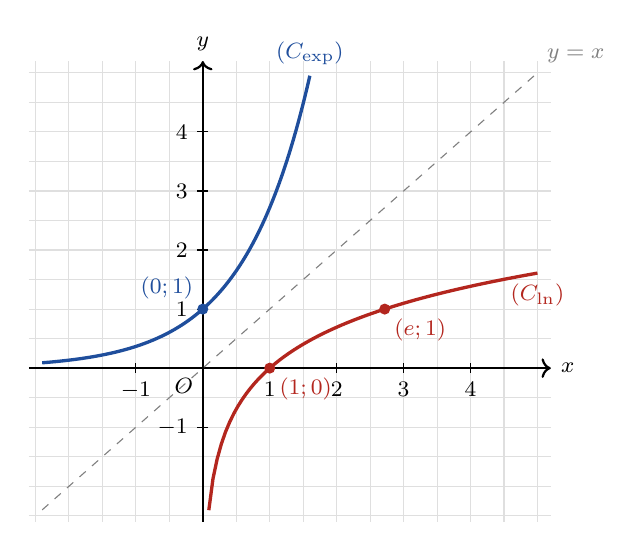
\begin{tikzpicture}[x=0.85cm,y=0.75cm,font=\footnotesize]\draw[gray!25,step=0.5] (-2.6,-2.6) grid (5.2,5.2);\draw[->,thick] (-2.6,0)--(5.2,0) node[right]{$x$}; \draw[->,thick] (0,-2.6)--(0,5.2) node[above]{$y$};\draw (-1,0.08)--(-1,-0.08) node[below]{$-1$};\draw (1,0.08)--(1,-0.08) node[below]{$1$};\draw (2,0.08)--(2,-0.08) node[below]{$2$};\draw (3,0.08)--(3,-0.08) node[below]{$3$};\draw (4,0.08)--(4,-0.08) node[below]{$4$};\draw (0.08,-1)--(-0.08,-1) node[left]{$-1$};\draw (0.08,1)--(-0.08,1) node[left]{$1$};\draw (0.08,2)--(-0.08,2) node[left]{$2$};\draw (0.08,3)--(-0.08,3) node[left]{$3$};\draw (0.08,4)--(-0.08,4) node[left]{$4$};\node[below left] at (0,0){$O$};\draw[gray,dashed] (-2.4,-2.4)--(5,5) node[above right]{$y=x$};
\draw[cDef,very thick,domain=-2.4:1.6,samples=80] plot (\x,{exp(\x)}) node[above]{$(C_{\exp})$};
\draw[cThm,very thick,domain=0.09:5,samples=80] plot (\x,{ln(\x)}) node[below]{$(C_{\ln})$};
\fill[cDef] (0,1) circle (2pt) node[above left]{$(0;1)$}; \fill[cThm] (1,0) circle (2pt) node[below right]{$(1;0)$};
\fill[cThm] (2.718,1) circle (2pt) node[below right]{$(e;1)$};\end{tikzpicture}\end{LTR}\par }{}{}
\Row{}{%
\Lab{cMeth}{حل معادلة أو متراجحة}\par\textbf{(1)} نعيّن مجموعة الحلول الممكنة $D$ (ما داخل $\ln$ موجب تمامًا).\par\textbf{(2)} نحوّل: $\ln u=\ln v$ تعني $u=v$ ؛ $\ln u=k$ تعني $u=e^k$ ؛ $\ln u<\ln v$ تعني $u<v$.\par\textbf{(3)} نأخذ الحلول التي تنتمي إلى $D$.}{}{}
\Row{}{%
\Lab{cEx}{أمثلة: حل في $\mathbb R$}\par\textbf{(1)} $\ln(2x+1)=0$: $D=\left]-\frac12;+\infty\right[$ ؛ $2x+1=e^0=1$ ، $x=0\in D$: $\RR{S=\{0\}}$.\par\textbf{(2)} $\ln(x-2)=-1$: $D=]2;+\infty[$ ؛ $x-2=e^{-1}$ ، $x=2+\dfrac1e\in D$: $\RR{S=\left\{2+\frac1e\right\}}$.\par\textbf{(3)} $\ln(x^2-1)=\ln x$: $D=]1;+\infty[$ ؛ $x^2-1=x$ ، أي $x^2-x-1=0$.\par الحلان $\dfrac{1-\sqrt5}2\notin D$ و $\dfrac{1+\sqrt5}2\approx1{,}62\in D$: $\RR{S=\left\{\frac{1+\sqrt5}2\right\}}$.\par\textbf{(4)} $e^{2x}-3e^x+2=0$: نضع $X=e^x>0$: $(X-1)(X-2)=0$ ، $e^x=1$ أو $e^x=2$: $\RR{S=\{0;\ln2\}}$.}{}{}
\Row{}{%
\Lab{cThm!80!black}{حذار}\ لا نحل قبل تعيين $D$ ، ولا ننسى التحقق أن الحلول تنتمي إليها.}{}{}
\Row{التقويم}{%
\Lab{cMeth}{تمرين تطبيقي}\par حل في $\mathbb R$ ما يلي:\par\textbf{(1)} $\ln(2-x)<0$.\par\textbf{(2)} $\ln(x-5)\geqslant-2$.\par\textbf{(3)} $\ln(2x+1)>\ln x$.\par\textbf{(4)} $x\ln x-\ln x\geqslant0$.\par\textbf{(5)} $2(\ln x)^2-\ln x-1=0$.}{25 د}{تقويم فردي.}
\Row{}{%
\Lab{cEx}{حل التمرين التطبيقي}\par\textbf{(1)} $D=]-\infty;2[$ ؛ $\ln(2-x)<\ln1$ تكافئ $2-x<1$ ، أي $x>1$: $\RR{S=]1;2[}$.\par\textbf{(2)} $D=]5;+\infty[$ ؛ $x-5\geqslant e^{-2}$ ، أي $x\geqslant5+e^{-2}$: $\RR{S=\left[5+e^{-2};+\infty\right[}$.\par\textbf{(3)} $D=]0;+\infty[$ ؛ $2x+1>x$ تكافئ $x>-1$ ، صحيحة على $D$: $\RR{S=]0;+\infty[}$.\par\textbf{(4)} $D=]0;+\infty[$ ؛ $(x-1)\ln x\geqslant0$ ، و $x-1$ و $\ln x$ لهما نفس الإشارة دائمًا (كلاهما سالب على $]0;1[$ وموجب على $]1;+\infty[$): $\RR{S=]0;+\infty[}$.\par\textbf{(5)} $D=]0;+\infty[$ ؛ نضع $X=\ln x$: $2X^2-X-1=0$ ، $X=1$ أو $X=-\dfrac12$.\par $\ln x=1$ يعني $x=e$ ؛ $\ln x=-\dfrac12$ يعني $x=e^{-\frac12}=\dfrac1{\sqrt e}$: $\RR{S=\left\{\frac1{\sqrt e};e\right\}}$.\par\textbf{واجب منزلي:} التمرينان 59 و 61 صفحة 106.\par\smallskip\textbf{ملاحظات حول سير الحصة:} \dotfill}{}{}
\end{Sayr}
\newpage
\ModhHead{15}{3 ع ت}{تحليل}{الدالة اللوغاريتمية النيبيرية}{02 سا}{الخواص الجبرية للدالة اللوغاريتمية}%
{\begin{itemize}\item تعريف الدالة $\ln$ ، خواص الدالة الأسية.\end{itemize}}%
{\begin{itemize}\item معرفة الخواص الجبرية للدالة $\ln$ وتوظيفها في الحساب وحل المعادلات والمتراجحات.\end{itemize}}%
{المنهاج ، الكتاب المدرسي ، الآلة الحاسبة العلمية ، برمجية Geogebra.}
\begin{Sayr}
\Row{مرحلة الانطلاق}{%
\textbf{التهيئة النفسية:} التذكير بخواص الدالة الأسية: $e^{x+y}=e^xe^y$ و $e^{nx}=(e^x)^n$.}{10 د}{تذكير.}
\Row{التشخيص والاكتشاف}{%
\Lab{cEx}{نشاط رقم 06}\ $a$ و $b$ عددان حقيقيان موجبان تمامًا. نضع $\alpha=\ln(ab)$ و $\beta=\ln a+\ln b$.\par\textbf{(1)} احسب $e^\alpha$ و $e^\beta$.\par\textbf{(2)} قارن بين $\alpha$ و $\beta$.}{35 د}{مناقشة النشاط.}
\Row{}{%
\Lab{cDef}{مناقشة النشاط}\par\textbf{(1)} $e^\alpha=e^{\ln(ab)}=ab$ ؛ $e^\beta=e^{\ln a+\ln b}=e^{\ln a}\times e^{\ln b}=ab$.\par\textbf{(2)} $e^\alpha=e^\beta$ ، إذن $\alpha=\beta$ ، أي $\RR{\ln(ab)=\ln a+\ln b}$.}{}{}
\Row{بناء المعارف}{%
\Lab{cThm}{الخاصية الأساسية}\ من أجل كل عددين $a$ و $b$ من $]0;+\infty[$: $\RR{\ln(a\times b)=\ln a+\ln b}$.\par (تعمم إلى جداء عدة أعداد موجبة تمامًا.)}{50 د}{البراهين مع التلاميذ.}
\Row{}{%
\Lab{cRem}{نتائج}\ من أجل كل $a>0$ و $b>0$ ومن أجل كل عدد صحيح $n$:\par\textbf{(1)} $\RR{\ln\dfrac1a=-\ln a}$ ؛ $\RR{\ln\dfrac ab=\ln a-\ln b}$.\par\textbf{(2)} $\RR{\ln\left(a^n\right)=n\ln a}$.\par\textbf{(3)} $\RR{\ln\sqrt a=\dfrac12\ln a}$.}{}{}
\Row{}{%
\Lab{cMeth}{البرهان}\par\textbf{(1)} $\ln a+\ln\dfrac1a=\ln\left(a\times\dfrac1a\right)=\ln1=0$ ، ومنه $\ln\dfrac1a=-\ln a$.\par $\ln\dfrac ab=\ln\left(a\times\dfrac1b\right)=\ln a+\ln\dfrac1b=\ln a-\ln b$.\par\textbf{(2)} $e^{n\ln a}=\left(e^{\ln a}\right)^n=a^n$ ، ومنه $\ln\left(a^n\right)=n\ln a$.\par\textbf{(3)} $a=\left(\sqrt a\right)^2$ ، إذن $\ln a=2\ln\sqrt a$ ، أي $\ln\sqrt a=\dfrac12\ln a$.}{}{}
\Row{}{%
\Lab{cEx}{أمثلة}\par\textbf{(1)} $\ln9=\ln3^2=\RR{2\ln3}$ ؛ $\ln8=\ln2^3=\RR{3\ln2}$ ؛ $\ln\sqrt e=\RR{\dfrac12}$.\par\textbf{(2)} $A=\ln12-\ln3=\ln\dfrac{12}3=\ln4=\RR{2\ln2}$.\par\textbf{(3)} $B=\ln\left(e^2\right)+\ln\dfrac1e=2-1=\RR{1}$.\par\textbf{(4)} $C=3\ln2+\ln\dfrac18=\ln8-\ln8=\RR{0}$.}{}{}
\Row{}{%
\Lab{cEx}{حل معادلة}\ $\ln x+\ln(x-2)=\ln3$: $D=]2;+\infty[$.\par\textbf{(1)} $\ln\big[x(x-2)\big]=\ln3$ ، أي $x^2-2x-3=0$ ، $(x-3)(x+1)=0$.\par\textbf{(2)} $x=3\in D$ و $x=-1\notin D$: $\RR{S=\{3\}}$.}{}{}
\Row{}{%
\Lab{cThm!80!black}{حذار}\ $\ln(a+b)\neq\ln a+\ln b$ ، و $\ln\dfrac ab\neq\dfrac{\ln a}{\ln b}$.}{}{}
\Row{التقويم}{%
\Lab{cMeth}{تمرين تطبيقي}\ (1)\par احسب بدلالة العدد الطبيعي $n\geqslant2$ المجموع: $S_n=\ln\dfrac12+\ln\dfrac23+\ln\dfrac34+\dots+\ln\dfrac{n-1}n$.}{25 د}{تقويم فردي.}
\Row{}{%
\Lab{cMeth}{تمرين تطبيقي 2}\par حل في $\mathbb R$:\par\textbf{(1)} $\ln(x-1)+\ln(x+2)\leqslant2\ln2$.\par\textbf{(2)} $\ln(x+1)-\ln(x-1)>0$.}{}{}
\Row{}{%
\Lab{cEx}{حل التمرين التطبيقي 1}\par $S_n=\ln\left(\dfrac12\times\dfrac23\times\dfrac34\times\dots\times\dfrac{n-1}n\right)$ (البسوط تختصر مع المقامات).\par $S_n=\ln\dfrac1n=\RR{-\ln n}$.}{}{}
\Row{}{%
\Lab{cEx}{حل التمرين التطبيقي 2}\par\textbf{(1)} $D=]1;+\infty[$ ؛ $\ln\big[(x-1)(x+2)\big]\leqslant\ln4$ ، أي $x^2+x-2\leqslant4$.\par $x^2+x-6\leqslant0$ ، $(x+3)(x-2)\leqslant0$ ، $-3\leqslant x\leqslant2$ ، مع $x>1$: $\RR{S=]1;2]}$.\par\textbf{(2)} $D=]1;+\infty[$ ؛ $\ln(x+1)>\ln(x-1)$ تكافئ $x+1>x-1$ ، صحيحة دائمًا: $\RR{S=]1;+\infty[}$.\par\textbf{واجب منزلي:} التمرينان 67 و 68 صفحة 107.\par\smallskip\textbf{ملاحظات حول سير الحصة:} \dotfill}{}{}
\end{Sayr}
\newpage
\ModhHead{16}{3 ع ت}{تحليل}{الدالة اللوغاريتمية النيبيرية}{02 سا}{اشتقاقية الدالة $\ln$ ودراسة الدالة $\ln\circ u$}%
{\begin{itemize}\item مشتقة دالة مركبة ، الدالة $\ln$ وخواصها.\end{itemize}}%
{\begin{itemize}\item حساب مشتقة الدالة $\ln$ ومشتقة الدالة $\ln\circ u$ ودراسة اتجاه تغيرها.\end{itemize}}%
{المنهاج ، الكتاب المدرسي ، الآلة الحاسبة العلمية ، برمجية Geogebra.}
\begin{Sayr}
\Row{مرحلة الانطلاق}{%
\textbf{التهيئة النفسية:} التذكير بمشتقة دالة مركبة.}{10 د}{تذكير.}
\Row{التشخيص والاكتشاف}{%
\Lab{cEx}{نشاط رقم 07}\ نقبل أن $\ln$ مستمرة وقابلة للاشتقاق على $]0;+\infty[$. نعتبر $f(x)=e^{\ln x}$ على $]0;+\infty[$.\par\textbf{(1)} احسب $f^{\prime}(x)$ باستعمال مشتقة مركب دالتين.\par\textbf{(2)} بملاحظة أن $f(x)=x$ ، احسب $f^{\prime}(x)$ مجددًا.\par\textbf{(3)} استنتج $\ln^{\prime}(x)$.}{35 د}{التلاميذ يبرهنون الخاصية.}
\Row{}{%
\Lab{cDef}{مناقشة النشاط}\par\textbf{(1)} $f^{\prime}(x)=\ln^{\prime}(x)\times e^{\ln x}=\ln^{\prime}(x)\times x$.\par\textbf{(2)} $f(x)=x$ ، إذن $f^{\prime}(x)=1$.\par\textbf{(3)} $x\,\ln^{\prime}(x)=1$ ، أي $\RR{\ln^{\prime}(x)=\dfrac1x}$.}{}{}
\Row{بناء المعارف}{%
\Lab{cThm}{خاصية 1}\ الدالة $\ln$ مستمرة على $]0;+\infty[$.}{50 د}{الوضع النسبي بجدول.}
\Row{}{%
\Lab{cThm}{خاصية 2}\ الدالة $\ln$ قابلة للاشتقاق على $]0;+\infty[$ و $\RR{\ln^{\prime}(x)=\dfrac1x}$.}{}{}
\Row{}{%
\Lab{cMeth}{المماس والوضع النسبي}\par\textbf{(1)} المماس عند $1$: $y=\ln^{\prime}(1)(x-1)+\ln1$ ، أي $\RR{(T):\ y=x-1}$.\par\textbf{(2)} نضع $g(x)=\ln x-(x-1)$: $g^{\prime}(x)=\dfrac1x-1=\dfrac{1-x}x$ ، موجبة على $]0;1[$ وسالبة على $]1;+\infty[$.\par\textbf{(3)} $g$ تبلغ قيمتها الحدية الكبرى $g(1)=0$ ، إذن $g(x)\leqslant0$ ، أي $\RR{\ln x\leqslant x-1}$:\par\smallskip\begin{LTR}\centering \begin{tikzpicture}[font=\normalsize]
\fill[gray!12] (0,0) rectangle (2.6,-0.9);
\fill[green!18] (2.6,0) rectangle (12.5,-0.9);
\fill[orange!45] (0,-0.9) rectangle (2.6,-4.6);
\fill[cyan!22] (2.6,-0.9) rectangle (12.5,-4.6);
\draw[thick] (0,0) rectangle (12.5,-4.6); \draw (0,-0.9)--(12.5,-0.9) (0,-1.8)--(12.5,-1.8) (2.6,0)--(2.6,-4.6);
\node at (1.3,-0.45){$x$};
\node at (1.3,-1.35){$\ln x-(x-1)$};
\node[align=center,font=\bfseries] at (1.3,-3.2){\ar{الوضع}\\ \ar{النسبي}};
\node at (3.3,-0.45){$0$};
\node at (7.55,-0.45){$1$};
\node at (11.8,-0.45){$+\infty$};
\node at (4.675,-1.35){$-$};
\node[align=center,font=\small] at (4.675,-3.2){$(C_{\ln})$\\ \ar{تحت}\\ $(T)$};
\node at (10.425,-1.35){$-$};
\node[align=center,font=\small] at (10.425,-3.2){$(C_{\ln})$\\ \ar{تحت}\\ $(T)$};
\node at (7.55,-1.35){$0$};
\draw[densely dotted] (7.55,-0.9)--(7.55,-1.13) (7.55,-1.57)--(7.55,-1.8);
\draw (6.05,-4.6) .. controls (6.125,-3.06) and (7.1,-2.136) .. (7.55,-1.8) .. controls (8,-2.136) and (8.975,-3.06) .. (9.05,-4.6);
\node[align=center,font=\footnotesize,inner sep=0pt] at (7.55,-3.65){\ar{$(C_{\ln})$ يمس}\\ $(T)$\\ \ar{في النقطة}\\ $A(1;0)$};
\end{tikzpicture}\end{LTR}\par }{}{}
\Row{}{%
\Lab{cThm}{اتجاه تغير $\ln\circ u$}\ إذا كانت $u$ معرفة وموجبة تمامًا على مجال $I$ فإن للدالتين $u$ و $\ln\circ u$ \RR{نفس} \RR{اتجاه} \RR{التغير} على $I$ (لأن $\ln$ متزايدة تمامًا).}{}{}
\Row{}{%
\Lab{cEx}{مثال}\ $f(x)=\ln\left(\dfrac5{x-2}\right)$ على $]2;+\infty[$: $u(x)=\dfrac5{x-2}$ متناقصة تمامًا وموجبة ، إذن \RR{$f$} \RR{متناقصة} \RR{تمامًا} \RR{على} \RR{$]2;+\infty[$}.}{}{}
\Row{}{%
\Lab{cThm}{المشتقة}\ إذا كانت $u$ قابلة للاشتقاق وموجبة تمامًا على $I$: $\RR{(\ln\circ u)^{\prime}(x)=\dfrac{u^{\prime}(x)}{u(x)}}$.}{}{}
\Row{}{%
\Lab{cMeth}{البرهان}\ حسب مشتقة مركب دالتين: $(\ln\circ u)^{\prime}(x)=u^{\prime}(x)\times\ln^{\prime}\big(u(x)\big)=u^{\prime}(x)\times\dfrac1{u(x)}$.}{}{}
\Row{}{%
\Lab{cEx}{أمثلة}\par\textbf{(1)} $f(x)=\ln\left(x^2+x+1\right)$ على $\mathbb R$ ($x^2+x+1>0$ لأن $\Delta=-3<0$): $\RR{f^{\prime}(x)=\dfrac{2x+1}{x^2+x+1}}$.\par\textbf{(2)} $g(x)=\ln\left(e^{-x}+3\right)$ على $\mathbb R$: $\RR{g^{\prime}(x)=\dfrac{-e^{-x}}{e^{-x}+3}}$.}{}{}
\Row{التقويم}{%
\Lab{cMeth}{تمرين تطبيقي}\par ادرس اتجاه تغير الدالة $f$ في كل حالة:\par\textbf{(1)} $f(x)=2x+\ln x$ ، $D_f=]0;+\infty[$.\par\textbf{(2)} $f(x)=x^2+2x+\ln(x+1)$ ، $D_f=]-1;+\infty[$.\par\textbf{(3)} $f(x)=x+5+6\ln\left(\dfrac x{x-1}\right)$ ، $D_f=]-\infty;0[$.\par\textbf{(4)} $f(x)=1+\dfrac{2\ln x}x$ ، $D_f=]0;+\infty[$.}{25 د}{تقويم فردي.}
\Row{}{%
\Lab{cEx}{حل التمرين التطبيقي}\par\textbf{(1)} $f^{\prime}(x)=2+\dfrac1x>0$ على $]0;+\infty[$: \RR{$f$} \RR{متزايدة} \RR{تمامًا}.\par\textbf{(2)} $f^{\prime}(x)=2x+2+\dfrac1{x+1}=2(x+1)+\dfrac1{x+1}>0$ لأن $x+1>0$: \RR{$f$} \RR{متزايدة} \RR{تمامًا}.\par\textbf{(3)} $u(x)=\dfrac x{x-1}>0$ على $]-\infty;0[$ (البسط والمقام سالبان).\par $\dfrac{u^{\prime}(x)}{u(x)}=\dfrac{-1}{(x-1)^2}\times\dfrac{x-1}x=\dfrac{-1}{x(x-1)}$.\par $f^{\prime}(x)=1-\dfrac6{x(x-1)}=\dfrac{x^2-x-6}{x(x-1)}=\dfrac{(x-3)(x+2)}{x(x-1)}$.\par على $]-\infty;0[$: $x(x-1)>0$ و $x-3<0$ ، فإشارة $f^{\prime}(x)$ عكس إشارة $x+2$:\par\smallskip\begin{LTR}\centering 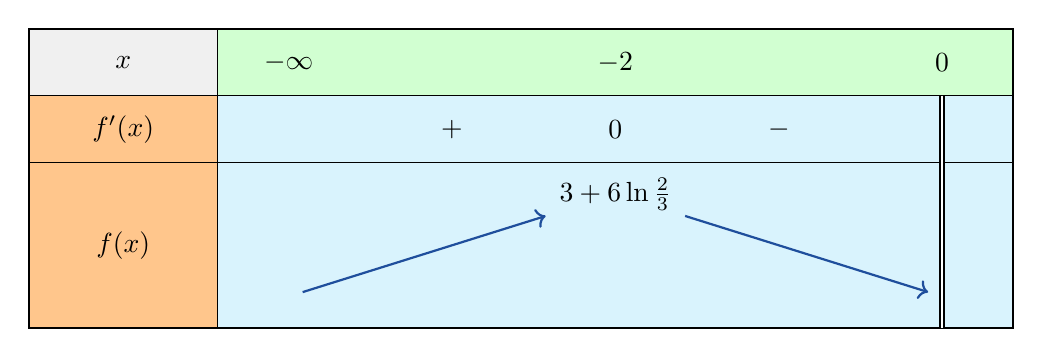
\begin{tikzpicture}[font=\normalsize]
\fill[gray!12] (0,0) rectangle (2.4,-0.85); \fill[green!18] (2.4,0) rectangle (12.5,-0.85);
\fill[orange!45] (0,-0.85) rectangle (2.4,-3.8); \fill[cyan!15] (2.4,-0.85) rectangle (12.5,-3.8);
\draw[thick] (0,0) rectangle (12.5,-3.8); \draw (0,-0.85)--(12.5,-0.85) (0,-1.7)--(12.5,-1.7) (2.4,0)--(2.4,-3.8);
\node at (1.2,-0.425){$x$}; \node at (1.2,-1.275){$f^{\prime}(x)$}; \node at (1.2,-2.75){$f(x)$};
\node at (3.3,-0.425){$-\infty$};
\node at (7.45,-0.425){$-2$};
\node at (11.6,-0.425){$0$};
\node at (5.375,-1.275){$+$};
\node at (7.45,-1.275){$0$};
\node at (9.525,-1.275){$-$};
\draw[double,thick] (11.6,-0.85)--(11.6,-3.8);
\node[inner sep=2pt] (v0) at (3.3,-3.4){$$};
\node[inner sep=2pt] (v1) at (7.45,-2.1){$3+6\ln\frac23$};
\node[inner sep=2pt] (v2) at (11.6,-3.4){$$};
\draw[->,cDef,thick,shorten <=3pt,shorten >=3pt] (v0)--(v1);
\draw[->,cDef,thick,shorten <=3pt,shorten >=3pt] (v1)--(v2);
\end{tikzpicture}\end{LTR}\par $f(-2)=3+6\ln\dfrac23\approx\RR{0{,}57}$.\par\textbf{(4)} $f^{\prime}(x)=\dfrac{2\times\frac1x\times x-2\ln x}{x^2}=\dfrac{2(1-\ln x)}{x^2}$.\par $f^{\prime}(x)>0$ يعني $\ln x<1$ ، أي $x<e$:\par\smallskip\begin{LTR}\centering 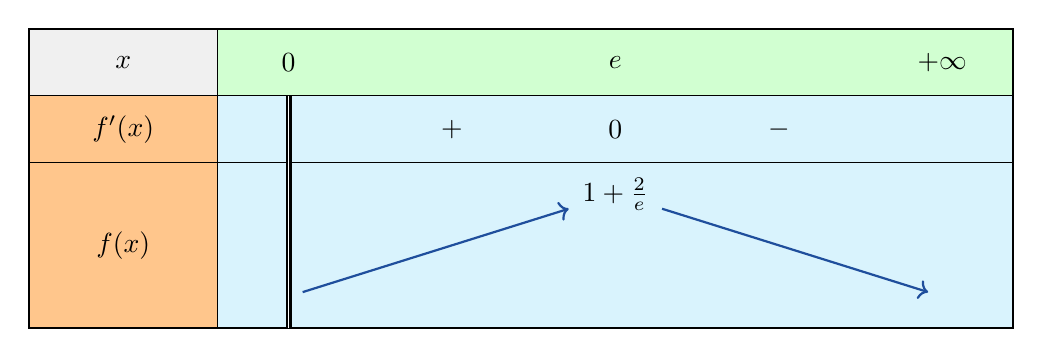
\begin{tikzpicture}[font=\normalsize]
\fill[gray!12] (0,0) rectangle (2.4,-0.85); \fill[green!18] (2.4,0) rectangle (12.5,-0.85);
\fill[orange!45] (0,-0.85) rectangle (2.4,-3.8); \fill[cyan!15] (2.4,-0.85) rectangle (12.5,-3.8);
\draw[thick] (0,0) rectangle (12.5,-3.8); \draw (0,-0.85)--(12.5,-0.85) (0,-1.7)--(12.5,-1.7) (2.4,0)--(2.4,-3.8);
\node at (1.2,-0.425){$x$}; \node at (1.2,-1.275){$f^{\prime}(x)$}; \node at (1.2,-2.75){$f(x)$};
\node at (3.3,-0.425){$0$};
\node at (7.45,-0.425){$e$};
\node at (11.6,-0.425){$+\infty$};
\draw[double,thick] (3.3,-0.85)--(3.3,-3.8);
\node at (5.375,-1.275){$+$};
\node at (7.45,-1.275){$0$};
\node at (9.525,-1.275){$-$};
\node[inner sep=2pt] (v0) at (3.3,-3.4){$$};
\node[inner sep=2pt] (v1) at (7.45,-2.1){$1+\frac2e$};
\node[inner sep=2pt] (v2) at (11.6,-3.4){$$};
\draw[->,cDef,thick,shorten <=3pt,shorten >=3pt] (v0)--(v1);
\draw[->,cDef,thick,shorten <=3pt,shorten >=3pt] (v1)--(v2);
\end{tikzpicture}\end{LTR}\par $f(e)=\RR{1+\dfrac2e}\approx1{,}74$.\par\textbf{واجب منزلي:} التمرينان 87 و 88 صفحة 108 ، والتمرينان 95 و 97 صفحة 109.\par\smallskip\textbf{ملاحظات حول سير الحصة:} \dotfill}{}{}
\end{Sayr}
\newpage
\ModhHead{17}{3 ع ت}{تحليل}{الدالة اللوغاريتمية النيبيرية}{02 سا}{اللوغاريتم العشري وتطبيقاته}%
{\begin{itemize}\item الدالة $\ln$ وخواصها الجبرية.\end{itemize}}%
{\begin{itemize}\item معرفة خواص دالة اللوغاريتم العشري وتطبيقاتها.\end{itemize}}%
{المنهاج ، الكتاب المدرسي ، الآلة الحاسبة العلمية ، برمجية Geogebra.}
\begin{Sayr}
\Row{مرحلة الانطلاق}{%
\textbf{التهيئة النفسية:} كم رقمًا يكتب به العدد $2^{100}$ ؟}{10 د}{سؤال تحفيزي.}
\Row{التشخيص والاكتشاف}{%
\Lab{cEx}{نشاط رقم 08}\ نعرف الدالة $\log$ على $]0;+\infty[$ بـ: $\log x=\dfrac{\ln x}{\ln10}$.\par\textbf{(1)} احسب $\log1$ و $\log10$ و $\log100$.\par\textbf{(2)} بيّن أن $\log(ab)=\log a+\log b$.\par\textbf{(3)} بيّن أن $\log10^n=n$ من أجل كل عدد صحيح $n$.}{35 د}{مناقشة النشاط.}
\Row{}{%
\Lab{cDef}{مناقشة النشاط}\par\textbf{(1)} $\log1=\dfrac0{\ln10}=\RR{0}$ ؛ $\log10=\RR{1}$ ؛ $\log100=\dfrac{2\ln10}{\ln10}=\RR{2}$.\par\textbf{(2)} $\log(ab)=\dfrac{\ln a+\ln b}{\ln10}=\RR{\log a+\log b}$.\par\textbf{(3)} $\log10^n=\dfrac{n\ln10}{\ln10}=\RR{n}$.}{}{}
\Row{بناء المعارف}{%
\Lab{cDef}{تعريف}\ دالة \textbf{اللوغاريتم العشري} هي الدالة $\log$ المعرفة على $]0;+\infty[$ بـ: $\RR{\log x=\dfrac{\ln x}{\ln10}}$.}{50 د}{تطبيقات من العلوم.}
\Row{}{%
\Lab{cThm}{خواص}\ من أجل كل $a>0$ و $b>0$ ومن أجل كل عدد صحيح $n$:\par\textbf{(1)} $\log(ab)=\log a+\log b$ ؛ $\log\dfrac ab=\log a-\log b$ ؛ $\log a^n=n\log a$.\par\textbf{(2)} $\RR{\log10^n=n}$.\par\textbf{(3)} $\log$ \RR{متزايدة} \RR{تمامًا} \RR{على} \RR{$]0;+\infty[$} لأن $\ln10>0$.}{}{}
\Row{}{%
\Lab{cRem}{نتيجة}\ إذا كان $10^n\leqslant x<10^{n+1}$ فإن $\RR{n\leqslant\log x<n+1}$.}{}{}
\Row{}{%
\Lab{cEx}{مثال}\ $x=3{,}87\times10^7$: $10^7<x<10^8$ ، إذن $\RR{7<\log x<8}$.}{}{}
\Row{}{%
\Lab{cMeth}{عدد أرقام عدد طبيعي $x\geqslant1$}\par\textbf{(1)} نحسب $\log x$ ونعيّن جزءه الصحيح $p$.\par\textbf{(2)} $p\leqslant\log x<p+1$ ، أي $10^p\leqslant x<10^{p+1}$.\par\textbf{(3)} عدد أرقام $x$ هو $\RR{p+1}$.}{}{}
\Row{}{%
\Lab{cEx}{تطبيق}\ عدد أرقام $n=2017^{2018}$:\par\textbf{(1)} $\log n=2018\log2017\approx6668{,}897$ ، الجزء الصحيح $6668$.\par\textbf{(2)} $10^{6668}\leqslant n<10^{6669}$: عدد الأرقام \RR{6669}.}{}{}
\Row{}{%
\Lab{cSec}{في الكيمياء}\ درجة الحموضة: $\RR{pH=-\log\left[H_3O^+\right]}$ (التركيز بـ $mol/L$). مثال: $\left[H_3O^+\right]=2{,}5\times10^{-4}$: $pH=-\log\left(2{,}5\times10^{-4}\right)\approx\RR{3{,}60}$.}{}{}
\Row{}{%
\Lab{cSec}{في الزلازل}\ درجة زلزال شدته $I$: $\RR{M=\log\dfrac I{I_0}}$ ($I_0$ شدة مرجعية). زلزال أشد بـ $10$ مرات: $\log\dfrac{10I}{I_0}=1+M$ ، أي \RR{تزيد} \RR{الدرجة} \RR{بـ} \RR{$1$}.}{}{}
\Row{التقويم}{%
\Lab{cMeth}{تمرين تطبيقي}\par\par\textbf{(1)} كم رقمًا يكتب به العدد $2^{100}$ ؟\par\textbf{(2)} احسب $pH$ محلول تركيزه $\left[H_3O^+\right]=4\times10^{-5}\ mol/L$.\par\textbf{(3)} حل في $\mathbb R$: $\log(2x+1)=1+\log(x-1)$.}{25 د}{نهاية المحور: فرض أو معالجة.}
\Row{}{%
\Lab{cEx}{حل التمرين التطبيقي}\par\textbf{(1)} $\log2^{100}=100\log2\approx30{,}103$ ، الجزء الصحيح $30$: عدد الأرقام \RR{31}.\par\textbf{(2)} $pH=-\log\left(4\times10^{-5}\right)=5-\log4\approx\RR{4{,}40}$.\par\textbf{(3)} $D=]1;+\infty[$ ؛ $1+\log(x-1)=\log\big[10(x-1)\big]$ ، إذن $2x+1=10x-10$ ، $x=\dfrac{11}8\in D$: $\RR{S=\left\{\frac{11}8\right\}}$.\par\textbf{واجب منزلي:} التمارين 98 و 100 و 101 صفحة 109.\par\smallskip\textbf{ملاحظات حول سير الحصة:} \dotfill}{}{}
\end{Sayr}
\end{document}
